\chapter{Contribution des CIOE dans une formulation équation intégrale}
\label{sec:equation_integrale}
\minitoc
\newpage
\sectionstar{Introduction}
Nous pouvons donc aborder la dernière partie de notre problème pour évaluer la pertinence de notre démarche. En effet, c'est en calculant les champs électromagnétiques tangentiels sur la surface de notre objet et en les comparants avec des résultats de référence.

Les équations intégrales sont des méthodes bien éprouvées pour résoudre les équations de Maxwell, tel que l'a démontré \cite{nedelec_acoustic_2001}. Ce chapitre rappelle quelques résultats connus et montre la contribution des \gls{acr-cioe}.

\section{Espaces fonctionnels}
  Les équations intégrales sont résolues grâce à la méthode des éléments finis de frontière. On rappelle dans cette partie des résultats connus nécessaires pour intégrer les CIOE.

  \begin{defn}
    Pour toute fonction \(\vect{U}(\vx) \in \Hrot(\OO_h), \vrot \vect{U}(\vx) \in L^2(\OO_h)\)

    Pour toute fonction \(\vect{U}(\vx) \in \Hdiv(\Gamma_h), \vdivs\vect{U}(\vx) \in L^2(\Gamma_h)\)

    Pour toute fonction \(\vect{U}(\vx) \in \Hrot(\Gamma_h), \vrots\vect{U}(\vx) \in L^2(\Gamma_h)\)
  \end{defn}
\section{Résolution des équations intégrales avec CIOE par la méthode des éléments finis de frontières}

  Les équations intégrales sont des méthodes bien éprouvées pour résoudre les équations de Maxwell, tel que l'a démontré \cite{nedelec_acoustic_2001}. Ce chapitre rappelle quelques résultats connus et montre la contribution des \gls{acr-cioe}.

  Les équations intégrales sont résolues grâce à la méthode des éléments finis de frontière.

  \subsection[Espace fonctionnel Hdiv]{Espace fonctionnel \(\Hdiv\)}
    On définit l'espace \(\Hdiv(\Gamma_h)\) tel que
    \begin{defn}
      Pour toute fonction \(\vect{U}(\vx) \in \Hdiv(\Gamma_h), \vdivs\vect{U}(\vx) \in L^2(\Gamma_h)\)
    \end{defn}

  \subsection{Équations intégrales}

      La démonstration de ces formules dépassent le cadre de cette thèse et nous renvoyons à \cite[\textsection~5.6]{nedelec_mixed_1980}.

      Soit \(G\) la fonction de Green défini en tout point extérieur à \(\Gamma_h\) telle que
      \begin{equation}
        G(\vz) = \frac{e^{-ik_0|\vz|}}{4\pi|\vz|}
      \end{equation}
      On définit \(g(\vx,\vy) := G(\vx - \vy)\).

      Soit \(\vE^{inc}_t,\vH^{inc}_t\) le champ incident tangentiel à \(\Gamma_h\). On définit le long de la surface \(\Gamma_h\), les traces tangentielles des champs \(\vJ = \vn \pvect \vH\), \(\vK = \vn \pvect \vE\).

      \subsubsection{EFIE}

        \begin{defn}
          \(\vJ,\vK\) sont solutions des équations intégrales en champ électrique (\gls{acr-efie}) si il existe \((\vJ,\vK) \in \Hdiv(\Gamma_h)^2\) tels que
          \begin{multline}
            \label{eq:form_int:EFIE}
            \vE^{inc}_t(\vx) =
              \frac{\vE_t(\vx)}{2}
                - \int_{\Gamma_h} \vgrad g(\vx - \vy) \pvect \vK(\vy) \dd{s}(\vy) \cdots \\
              + \frac{i}{k}\vgrad \int_{\Gamma_h}  g(\vx - \vy)\vdiv\vJ(\vy)(\vx) \dd{s}(\vy)
                +  ik\int_{\Gamma_h} g(\vx - \vy)\vJ(\vy) \dd{s}(\vy)
          \end{multline}
        \end{defn}


      \subsubsection{MFIE}

        \begin{defn}
          \(\vJ,\vK\) sont solutions des équations intégrales en champ magnétique (\gls{acr-mfie}) si il existe \((\vJ,\vK) \in \Hdiv(\Gamma_h)^2\) tels que
          \begin{multline}
            \label{eq:form_int:MFIE}
            \vH^{inc}(\vx) =
            \frac{\vH_t(\vx)}{2}
              - \int_{\Gamma_h} \vgrad g(\vx - \vy) \pvect \vJ(\vy) \dd{s}(\vy) \cdots \\
            - \frac{i}{k} \vgrad \int_{\Gamma_h}  g(\vx - \vy)\vdiv\vK(\vy)\dd{s}(\vy)
              - ik \int_{\Gamma_h} g(\vx - \vy)\vK(\vy)\dd{s}(\vy)
          \end{multline}
        \end{defn}

  \subsection{Discrétisation de la surface de l'objet}

    La méthode numérique utilisé au CEA depuis les années 90 est basé sur l'article de \cite{medgyesi-mitschang_integral_1985}. Nous rappelons cette méthode en conservant les notations de \cite{stupfel_implementation_2015}.\\

    Soit \(\Gamma_h\) un maillage fermé de \(\Gamma\) en \(N_e\) éléments triangulaires. Soit \(N=\frac{3}{2}N_e\) le nombre d'arête du maillage. On désigne par \(\vn\) la normale unitaire sortante du maillage, non défini aux nœuds et arêtes du maillage.

    Soit \(T\) un triangle défini par un nœud \(N_1\) et deux vecteurs \(\vect{e_1}\) et \(\vect{e_2}\). On rappelle la relation entre l'aire du triangle et ces vecteurs
    \begin{equation}
      2|T| = |\vect{e_1}\pvect\vect{e_2}|
    \end{equation}

    % Les commandes qui suivent servent pour les prochains schémas
    \newcommand{\ncouche}{6}
    \newcommand{\setnodes}[6]{
        \renewcommand{\xa}{#1}
        \renewcommand{\ya}{#2}
        \renewcommand{\xb}{#3}
        \renewcommand{\yb}{#4}
        \renewcommand{\xc}{#5}
        \renewcommand{\yc}{#6}
    }
    \newcommand{\xa}{0.0}
    \newcommand{\ya}{0.0}
    \newcommand{\xb}{3.0}
    \newcommand{\yb}{0.0}
    \newcommand{\xc}{0.0}
    \newcommand{\yc}{3.0}
    \begin{minipage}{0.45\textwidth}
      \begin{center}
        \tikzsetnextfilename{fonbasloc_triangle_loc}
        \begin{tikzpicture}[scale=1]
          %%% Triangle de gauche

%%% Triangle de gauche

\coordinate (na) at (\xa,\ya);
\coordinate (nb) at (\xb,\yb);
\coordinate (nc) at (\xc,\yc);

\coordinate (ec) at ($(nb)-(na)$);
\coordinate (ea) at ($(nc)-(nb)$);

\draw (na) -- (nc) -- (nb) -- cycle;


%\draw [-Latex] (n3) -- (n2) node [midway,above right] {\(\vect{e_1}\)};
\draw [-Latex] (n1) -- (n3) node [midway,below] {\(\vect{e_1}\)};
\draw [-Latex] (n1) -- (n2) node [midway,left] {\(\vect{e_2}\)};

\draw [-Latex] (n2) -- (n3) node [midway,above,sloped] {\(\vect{u_j}\)};

\coordinate (pt) at  ($1/3*(n1)+1/3*(n2)+1/3*(n3)$);

\draw (pt) node {\(T\)};

\newcommand{\nutau}[3]{
  % la normale nu
  \path let \p1=(#1) in coordinate (nu) at (\y1,-\x1);

  \tikzmath
  {
      \ra = sqrt((\xb-\xc)^2 + (\yb-\yc)^2);
  }

  \draw [-Latex] (#2) -- ($(#2) + 1/\ra*(nu)$) node [midway,below,sloped] {\(\vect{\nu_{#3}}\)};

  % % la normale tau_j
  \path let \p1=(nu) in coordinate (tau) at (-\y1,\x1);
  \draw [-Latex] (#2) -- ($(#2) + 1/\ra*(tau)$) node [midway,above,sloped] {\(\vect{\tau_{#3}}\)};
}

% \nutau{e1}{$1/3*(n2)+2/3*(n3)$}{1}
% \nutau{e2}{n1}{2}
% \nutau{e3}{n2}{3}

% La normale au triangle.
\coordinate (pn) at  ($3/4*(n1)+1/8*(n2)+1/8*(n3)$);
\draw[thick] (pn) circle(0.1) node [right=0.6] {\(\vn\)};
\fill (pn) circle(0.03);


\draw (n1) node [below left] {\(N_1\)};
%\draw (n2) node [above left] {\(N_2\)};
%\draw (n3) node [below right] {\(N_3\)};

        \end{tikzpicture}
      \end{center}
      \captionof{figure}{Triangles, arêtes et nœuds définis par l'arête \(\uj\)}
      \label{fig:form_int:fon_base:tri}
    \end{minipage}
    \begin{minipage}{0.54\textwidth}
     On se place dans le repère local au triangle, on fait donc les changement de coordonnées suivant:
    \begin{align*}
      \RR^3 &\rightarrow [0,1]^2 \\
      (x_1,x_2,x_3) & \mapsto (\xi_1,\xi_2)
    \end{align*}
      tel que \(\vx =\vect{N_1}+ \xi_1 \vect{e_1} + \xi_2 \vect{e_2}\).
    \end{minipage}

    \subsubsection[Fonctions de Raviart-Thomas phi Hdiv-conforme]{Fonctions de Raviart-Thomas \(\vect{\phi}\) \(\Hdiv\)-conforme}

      Ces fonctions ont été introduites par \cite{raviart_mixed_1977}. Nous présentons ici les fonctions Raviart-Thomas de degré 0, c'est à dire telles que les degrés de libertés soient au milieu de chaque arête (voir \cite[eq.~(3.10)]{raviart_mixed_1977}).

      \begin{minipage}{\textwidth}
        \begin{minipage}{0.329\textwidth}
            % Les commandes qui suivent servent pour les 4 prochains schémas
            \setnodes{0}{0}{3}{0}{0}{3}
            \begin{center}
              \tikzsetnextfilename{fonbasloc_phi_1}
              \begin{tikzpicture}[scale=1]
                %%% Triangle de gauche

\tikzmath
{
    \ra = sqrt((\xb-\xc)^2 + (\yb-\yc)^2);
    \rb = sqrt((\xc-\xa)^2 + (\yc-\ya)^2);
    \rc = sqrt((\xa-\xb)^2 + (\ya-\yb)^2);
    \aire = 0.25*sqrt((\ra+\rb-\rc)*(\ra-\rb+\rc)*(-\ra+\rb+\rc)*(\ra+\rb+\rc));
}

\coordinate (na) at (\xa,\ya);
\coordinate (nb) at (\xb,\yb);
\coordinate (nc) at (\xc,\yc);

\coordinate (ec) at ($(nb)-(na)$);
\coordinate (ea) at ($(nc)-(nb)$);

\draw (na) -- (nc) -- (nb) -- cycle;

\foreach \couche in {1,...,\ncouche}
{
    \tikzmath
    {
        \a = \couche/\ncouche;
    }
    \foreach \n in {0,...,\couche}
    {
        \tikzmath
        {
            \b = \n/\couche;
        }
        \coordinate (phi) at ($\a*(ec)+\a*\b*(ea)$);
        \coordinate (x) at ($(na)+(phi)$);
        % \draw (x) node {\(x_\n^\couche\)};
        \draw [->] (x) -- ($(x)+1/\aire*(phi)$);
    }
}

%%% Triangle de droite

\tikzmath
{
    \rd = sqrt((\xb-\xc)^2 + (\yb-\yc)^2);
    \rb = sqrt((\xc-\xd)^2 + (\yc-\yd)^2);
    \rc = sqrt((\xd-\xb)^2 + (\yd-\yb)^2);
    \aire = 0.25*sqrt((\rd+\rb-\rc)*(\rd-\rb+\rc)*(-\rd+\rb+\rc)*(\rd+\rb+\rc));
}

\coordinate (nd) at (\xd,\yd);

\coordinate (ed) at ($(nc)-(nb)$);
\coordinate (ec) at ($(nb)-(nd)$);

\draw (nb) -- (nd) -- (nc) -- cycle;

\foreach \couche in {1,...,\ncouche}
{
    \tikzmath
    {
        \a = \couche/\ncouche;
    }
    \foreach \n in {0,...,\couche}
    {
        \tikzmath
        {
            \b = \n/\couche;
        }
        \coordinate (phi) at ($\a*(ec)+\a*\b*(ed)$);
        \coordinate (x) at ($(nd)+(phi)$);
        % \draw (x) node {\(x_\n^\couche\)};
        \draw [->] (x) -- ($(x)-1/\aire*(phi)$);
    }
}

              \end{tikzpicture}
            \end{center}
            \begin{equation*}
              \vect{\phi_1}=\frac{\xi_1}{2|T|}\vect{e_1} + \frac{\xi_2}{{2|T|}}\vect{e_2}
            \end{equation*}
        \end{minipage}
        \begin{minipage}{0.329\textwidth}
            \setnodes{3}{0}{0}{3}{0}{0}
            \begin{center}
              \tikzsetnextfilename{fonbasloc_phi_2}
              \begin{tikzpicture}[scale=1]
                %%% Triangle de gauche

\tikzmath
{
    \ra = sqrt((\xb-\xc)^2 + (\yb-\yc)^2);
    \rb = sqrt((\xc-\xa)^2 + (\yc-\ya)^2);
    \rc = sqrt((\xa-\xb)^2 + (\ya-\yb)^2);
    \aire = 0.25*sqrt((\ra+\rb-\rc)*(\ra-\rb+\rc)*(-\ra+\rb+\rc)*(\ra+\rb+\rc));
}

\coordinate (na) at (\xa,\ya);
\coordinate (nb) at (\xb,\yb);
\coordinate (nc) at (\xc,\yc);

\coordinate (ec) at ($(nb)-(na)$);
\coordinate (ea) at ($(nc)-(nb)$);

\draw (na) -- (nc) -- (nb) -- cycle;

\foreach \couche in {1,...,\ncouche}
{
    \tikzmath
    {
        \a = \couche/\ncouche;
    }
    \foreach \n in {0,...,\couche}
    {
        \tikzmath
        {
            \b = \n/\couche;
        }
        \coordinate (phi) at ($\a*(ec)+\a*\b*(ea)$);
        \coordinate (x) at ($(na)+(phi)$);
        % \draw (x) node {\(x_\n^\couche\)};
        \draw [->] (x) -- ($(x)+1/\aire*(phi)$);
    }
}

%%% Triangle de droite

\tikzmath
{
    \rd = sqrt((\xb-\xc)^2 + (\yb-\yc)^2);
    \rb = sqrt((\xc-\xd)^2 + (\yc-\yd)^2);
    \rc = sqrt((\xd-\xb)^2 + (\yd-\yb)^2);
    \aire = 0.25*sqrt((\rd+\rb-\rc)*(\rd-\rb+\rc)*(-\rd+\rb+\rc)*(\rd+\rb+\rc));
}

\coordinate (nd) at (\xd,\yd);

\coordinate (ed) at ($(nc)-(nb)$);
\coordinate (ec) at ($(nb)-(nd)$);

\draw (nb) -- (nd) -- (nc) -- cycle;

\foreach \couche in {1,...,\ncouche}
{
    \tikzmath
    {
        \a = \couche/\ncouche;
    }
    \foreach \n in {0,...,\couche}
    {
        \tikzmath
        {
            \b = \n/\couche;
        }
        \coordinate (phi) at ($\a*(ec)+\a*\b*(ed)$);
        \coordinate (x) at ($(nd)+(phi)$);
        % \draw (x) node {\(x_\n^\couche\)};
        \draw [->] (x) -- ($(x)-1/\aire*(phi)$);
    }
}

              \end{tikzpicture}
               \begin{equation*}
                \vect{\phi_2}=\frac{\xi_1-1}{2|T|}\vect{e_1} + \frac{\xi_2}{2|T|}\vect{e_2}
              \end{equation*}
            \end{center}
        \end{minipage}
        \begin{minipage}{0.329\textwidth}
            \setnodes{0}{3}{0}{0}{3}{0}
            \begin{center}
              \tikzsetnextfilename{fonbasloc_phi_3}            
              \begin{tikzpicture}[scale=1]
                %%% Triangle de gauche

\tikzmath
{
    \ra = sqrt((\xb-\xc)^2 + (\yb-\yc)^2);
    \rb = sqrt((\xc-\xa)^2 + (\yc-\ya)^2);
    \rc = sqrt((\xa-\xb)^2 + (\ya-\yb)^2);
    \aire = 0.25*sqrt((\ra+\rb-\rc)*(\ra-\rb+\rc)*(-\ra+\rb+\rc)*(\ra+\rb+\rc));
}

\coordinate (na) at (\xa,\ya);
\coordinate (nb) at (\xb,\yb);
\coordinate (nc) at (\xc,\yc);

\coordinate (ec) at ($(nb)-(na)$);
\coordinate (ea) at ($(nc)-(nb)$);

\draw (na) -- (nc) -- (nb) -- cycle;

\foreach \couche in {1,...,\ncouche}
{
    \tikzmath
    {
        \a = \couche/\ncouche;
    }
    \foreach \n in {0,...,\couche}
    {
        \tikzmath
        {
            \b = \n/\couche;
        }
        \coordinate (phi) at ($\a*(ec)+\a*\b*(ea)$);
        \coordinate (x) at ($(na)+(phi)$);
        % \draw (x) node {\(x_\n^\couche\)};
        \draw [->] (x) -- ($(x)+1/\aire*(phi)$);
    }
}

%%% Triangle de droite

\tikzmath
{
    \rd = sqrt((\xb-\xc)^2 + (\yb-\yc)^2);
    \rb = sqrt((\xc-\xd)^2 + (\yc-\yd)^2);
    \rc = sqrt((\xd-\xb)^2 + (\yd-\yb)^2);
    \aire = 0.25*sqrt((\rd+\rb-\rc)*(\rd-\rb+\rc)*(-\rd+\rb+\rc)*(\rd+\rb+\rc));
}

\coordinate (nd) at (\xd,\yd);

\coordinate (ed) at ($(nc)-(nb)$);
\coordinate (ec) at ($(nb)-(nd)$);

\draw (nb) -- (nd) -- (nc) -- cycle;

\foreach \couche in {1,...,\ncouche}
{
    \tikzmath
    {
        \a = \couche/\ncouche;
    }
    \foreach \n in {0,...,\couche}
    {
        \tikzmath
        {
            \b = \n/\couche;
        }
        \coordinate (phi) at ($\a*(ec)+\a*\b*(ed)$);
        \coordinate (x) at ($(nd)+(phi)$);
        % \draw (x) node {\(x_\n^\couche\)};
        \draw [->] (x) -- ($(x)-1/\aire*(phi)$);
    }
}

              \end{tikzpicture}
              \begin{equation*}
                \vect{\phi_3}=\frac{\xi_1}{2|T|}\vect{e_1} + \frac{\xi_2-1}{2|T|}\vect{e_2}
              \end{equation*}
            \end{center}
        \end{minipage}
        \captionof{figure}{Fonctions \(\phij\) locales}
        \label{fig:form_int:fon_base:phi}
      \end{minipage}

      \begin{prop}
        Les fonctions \(\phij\) sont dans \(\Hdiv(\Gamma_h)\)
      \end{prop}
      \begin{proof}
        Concernant la relation de compatibilité \(\Hdiv\), nous renvoyons à la propriété~\ref{prop:annex:hdiv_hrot:hdiv} en annexe.
      \end{proof}

      \begin{defn}
        Pour tout \(\vect{U} \in \Hdiv(\Gamma_h)\), alors
        \begin{equation*}
          \vect{U} \in \Vect{\vect{\phi_1},\ldots,\vect{\phi_N}} \Leftrightarrow \exists \comp{u} = (u_1,\cdots,u_N)^t \in \RR^N, \vect{U}(\vx) = \sum_{j=1}^N u_j \phij(\vx)
        \end{equation*}
      \end{defn}
  %%%%%%%%%%%%%%%%%%%%%%%%%%%%%%%%%%%%%%%%%%%%%%%%%%%%%%%%%%%%%%%%%%%%%%%%%%%%%%%%%%%%%%%%%%%%%%%%%%%%%%%%
  %%%%%%%%%%%%%%%%%%%%%%%%%%%%%%%%%%%%%%%%%%%%%%%%%%%%%%%%%%%%%%%%%%%%%%%%%%%%%%%%%%%%%%%%%%%%%%%%%%%%%%%%
  %%%%%%%%%%%%%%%%%%%%%%%%%%%%%%%%%%%%%%%%%%%%%%%%%%%%%%%%%%%%%%%%%%%%%%%%%%%%%%%%%%%%%%%%%%%%%%%%%%%%%%%%

  \subsection{Fonctions de projections}


    \subsubsection[Fonctions de Nédélec p Hrot-conforme]{Fonctions de Nédelec \(\vect{p}\) \(\Hrot\)-conforme}

      Une première famille est celle des \(\pj=-\vn\pvect\phij\), où la normale est défini dans un triangle. On les nomme fonctions de Nédélec car elles correspondent en 2D aux fonctions volumiques de Nédélec (voir \cite{nedelec_mixed_1980}).

      \begin{minipage}{\textwidth}
        \begin{minipage}{0.329\textwidth}
            % Les commandes qui suivent servent pour les 4 prochains schémas
            \setnodes{0}{0}{3}{0}{0}{3}
            \begin{center}
              \tikzsetnextfilename{fonbasloc_p_1}
              \begin{tikzpicture}[scale=1]
                %%% Triangle de gauche

\tikzmath
{
    \ra = sqrt((\xb-\xc)^2 + (\yb-\yc)^2);
    \rb = sqrt((\xc-\xa)^2 + (\yc-\ya)^2);
    \rc = sqrt((\xa-\xb)^2 + (\ya-\yb)^2);
    \aire = 0.25*sqrt((\ra+\rb-\rc)*(\ra-\rb+\rc)*(-\ra+\rb+\rc)*(\ra+\rb+\rc));
}

\coordinate (na) at (\xa,\ya);
\coordinate (nb) at (\xb,\yb);
\coordinate (nc) at (\xc,\yc);

\coordinate (ec) at ($(nb)-(na)$);
\coordinate (ea) at ($(nc)-(nb)$);

\draw (na) -- (nc) -- (nb) -- cycle;

\foreach \couche in {1,...,\ncouche}
{
    \tikzmath
    {
        \a = \couche/\ncouche;
    }
    \foreach \n in {0,...,\couche}
    {
        \tikzmath
        {
            \b = \n/\couche;
        }
        \coordinate (phi) at ($\a*(ec)+\a*\b*(ea)$);
        \coordinate (x) at ($(na)+(phi)$);
        \path let \p1=(phi) in coordinate (p) at (\y1,-\x1);
        % \draw (x) node {\(x_\n^\couche\)};
        \draw [->] (x) -- ($(x)+1/\aire*(p)$);
    }
}

%%% Triangle de droite

\tikzmath
{
    \rd = sqrt((\xb-\xc)^2 + (\yb-\yc)^2);
    \rb = sqrt((\xc-\xd)^2 + (\yc-\yd)^2);
    \rc = sqrt((\xd-\xb)^2 + (\yd-\yb)^2);
    \aire = 0.25*sqrt((\rd+\rb-\rc)*(\rd-\rb+\rc)*(-\rd+\rb+\rc)*(\rd+\rb+\rc));
}

\coordinate (nd) at (\xd,\yd);

\coordinate (ed) at ($(nc)-(nb)$);
\coordinate (ec) at ($(nb)-(nd)$);

\draw (nb) -- (nd) -- (nc) -- cycle;

\foreach \couche in {1,...,\ncouche}
{
    \tikzmath
    {
        \a = \couche/\ncouche;
    }
    \foreach \n in {0,...,\couche}
    {
        \tikzmath
        {
            \b = \n/\couche;
        }
        \coordinate (phi) at ($\a*(ec)+\a*\b*(ed)$);
        \coordinate (x) at ($(nd)+(phi)$);
        \path let \p1=(phi) in coordinate (p) at (\y1,-\x1);
        % \draw (x) node {\(x_\n^\couche\)};
        \draw [->] (x) -- ($(x)-1/\aire*(p)$);
    }
}

              \end{tikzpicture}
            \end{center}
            \begin{equation*}
              \vect{p_1}=\frac{\xi_2}{2|T|}\vect{e_1}-\frac{\xi_1}{2|T|}\vect{e_2}
            \end{equation*}
        \end{minipage}
        \begin{minipage}{0.329\textwidth}
            \setnodes{3}{0}{0}{3}{0}{0}
            \begin{center}
              \tikzsetnextfilename{fonbasloc_p_2}
              \begin{tikzpicture}[scale=1]
                %%% Triangle de gauche

\tikzmath
{
    \ra = sqrt((\xb-\xc)^2 + (\yb-\yc)^2);
    \rb = sqrt((\xc-\xa)^2 + (\yc-\ya)^2);
    \rc = sqrt((\xa-\xb)^2 + (\ya-\yb)^2);
    \aire = 0.25*sqrt((\ra+\rb-\rc)*(\ra-\rb+\rc)*(-\ra+\rb+\rc)*(\ra+\rb+\rc));
}

\coordinate (na) at (\xa,\ya);
\coordinate (nb) at (\xb,\yb);
\coordinate (nc) at (\xc,\yc);

\coordinate (ec) at ($(nb)-(na)$);
\coordinate (ea) at ($(nc)-(nb)$);

\draw (na) -- (nc) -- (nb) -- cycle;

\foreach \couche in {1,...,\ncouche}
{
    \tikzmath
    {
        \a = \couche/\ncouche;
    }
    \foreach \n in {0,...,\couche}
    {
        \tikzmath
        {
            \b = \n/\couche;
        }
        \coordinate (phi) at ($\a*(ec)+\a*\b*(ea)$);
        \coordinate (x) at ($(na)+(phi)$);
        \path let \p1=(phi) in coordinate (p) at (\y1,-\x1);
        % \draw (x) node {\(x_\n^\couche\)};
        \draw [->] (x) -- ($(x)+1/\aire*(p)$);
    }
}

%%% Triangle de droite

\tikzmath
{
    \rd = sqrt((\xb-\xc)^2 + (\yb-\yc)^2);
    \rb = sqrt((\xc-\xd)^2 + (\yc-\yd)^2);
    \rc = sqrt((\xd-\xb)^2 + (\yd-\yb)^2);
    \aire = 0.25*sqrt((\rd+\rb-\rc)*(\rd-\rb+\rc)*(-\rd+\rb+\rc)*(\rd+\rb+\rc));
}

\coordinate (nd) at (\xd,\yd);

\coordinate (ed) at ($(nc)-(nb)$);
\coordinate (ec) at ($(nb)-(nd)$);

\draw (nb) -- (nd) -- (nc) -- cycle;

\foreach \couche in {1,...,\ncouche}
{
    \tikzmath
    {
        \a = \couche/\ncouche;
    }
    \foreach \n in {0,...,\couche}
    {
        \tikzmath
        {
            \b = \n/\couche;
        }
        \coordinate (phi) at ($\a*(ec)+\a*\b*(ed)$);
        \coordinate (x) at ($(nd)+(phi)$);
        \path let \p1=(phi) in coordinate (p) at (\y1,-\x1);
        % \draw (x) node {\(x_\n^\couche\)};
        \draw [->] (x) -- ($(x)-1/\aire*(p)$);
    }
}

              \end{tikzpicture}
               \begin{equation*}
                \vect{p_2}= \frac{\xi_2}{2|T|}\vect{e_1} + \frac{1-\xi_1}{2|T|}\vect{e_2}
              \end{equation*}
            \end{center}
        \end{minipage}
        \begin{minipage}{0.329\textwidth}
            \setnodes{0}{3}{0}{0}{3}{0}
            \begin{center}
              \tikzsetnextfilename{fonbasloc_p_3}
              \begin{tikzpicture}[scale=1]
                %%% Triangle de gauche

\tikzmath
{
    \ra = sqrt((\xb-\xc)^2 + (\yb-\yc)^2);
    \rb = sqrt((\xc-\xa)^2 + (\yc-\ya)^2);
    \rc = sqrt((\xa-\xb)^2 + (\ya-\yb)^2);
    \aire = 0.25*sqrt((\ra+\rb-\rc)*(\ra-\rb+\rc)*(-\ra+\rb+\rc)*(\ra+\rb+\rc));
}

\coordinate (na) at (\xa,\ya);
\coordinate (nb) at (\xb,\yb);
\coordinate (nc) at (\xc,\yc);

\coordinate (ec) at ($(nb)-(na)$);
\coordinate (ea) at ($(nc)-(nb)$);

\draw (na) -- (nc) -- (nb) -- cycle;

\foreach \couche in {1,...,\ncouche}
{
    \tikzmath
    {
        \a = \couche/\ncouche;
    }
    \foreach \n in {0,...,\couche}
    {
        \tikzmath
        {
            \b = \n/\couche;
        }
        \coordinate (phi) at ($\a*(ec)+\a*\b*(ea)$);
        \coordinate (x) at ($(na)+(phi)$);
        \path let \p1=(phi) in coordinate (p) at (\y1,-\x1);
        % \draw (x) node {\(x_\n^\couche\)};
        \draw [->] (x) -- ($(x)+1/\aire*(p)$);
    }
}

%%% Triangle de droite

\tikzmath
{
    \rd = sqrt((\xb-\xc)^2 + (\yb-\yc)^2);
    \rb = sqrt((\xc-\xd)^2 + (\yc-\yd)^2);
    \rc = sqrt((\xd-\xb)^2 + (\yd-\yb)^2);
    \aire = 0.25*sqrt((\rd+\rb-\rc)*(\rd-\rb+\rc)*(-\rd+\rb+\rc)*(\rd+\rb+\rc));
}

\coordinate (nd) at (\xd,\yd);

\coordinate (ed) at ($(nc)-(nb)$);
\coordinate (ec) at ($(nb)-(nd)$);

\draw (nb) -- (nd) -- (nc) -- cycle;

\foreach \couche in {1,...,\ncouche}
{
    \tikzmath
    {
        \a = \couche/\ncouche;
    }
    \foreach \n in {0,...,\couche}
    {
        \tikzmath
        {
            \b = \n/\couche;
        }
        \coordinate (phi) at ($\a*(ec)+\a*\b*(ed)$);
        \coordinate (x) at ($(nd)+(phi)$);
        \path let \p1=(phi) in coordinate (p) at (\y1,-\x1);
        % \draw (x) node {\(x_\n^\couche\)};
        \draw [->] (x) -- ($(x)-1/\aire*(p)$);
    }
}

              \end{tikzpicture}
              \begin{equation*}
                \vect{p_3}= \frac{\xi_2-1}{2|T|}\vect{e_1} - \frac{\xi_1}{2|T|}\vect{e_2}
              \end{equation*}
            \end{center}
        \end{minipage}
        \captionof{figure}{Fonctions \(\pj\) locales}
        \label{fig:form_int:fon_base:p}
      \end{minipage}

      \begin{prop}
        Les fonctions \(\pj\) sont dans \(\Hrot(\Gamma_h)\)
      \end{prop}
      \begin{proof}
        Nous renvoyons au travail de \cite{nedelec_mixed_1980} (voir Annexe prop.~\ref{prop:annex:hdiv_hrot:hrot}).
      \end{proof}


      \begin{defn}
        Pour tout \(\vect{V} \in \Hrot(\Gamma_h)\), alors
        \begin{equation*}
          \vect{V} \in \Vect{\vect{p_1},\ldots,\vect{p_N}} \Leftrightarrow \exists \comp{v} = (v_1,\cdots,v_N)^t \in \RR^N, \vect{V}(\vx) = \sum_{j=1}^N v_j \pj(\vx)
        \end{equation*}
      \end{defn}

    \subsubsection[Fonctions de Bendali q]{Fonctions de Bendali \(\vect{q}\)}

      Ces fonctions ont été introduites par \cite[eq.~28]{bendali_boundary-element_1999}. Elles sont linéairement indépendantes. Nous modifions ces fonctions en les divisant par 2 fois l'aire du triangle. Ainsi, la matrice de passage (défini plus tard) sera plus simple.


      \begin{minipage}{\textwidth}
        \begin{minipage}{0.329\textwidth}
            % Les commandes qui suivent servent pour les 4 prochains schémas
            \setnodes{0}{0}{3}{0}{0}{3}
            \begin{center}
              \tikzsetnextfilename{fonbasloc_q_1}
              \begin{tikzpicture}[scale=1]
                %%% Triangle de gauche
%%% Triangle de gauche

\coordinate (na) at (\xa,\ya);
\coordinate (nb) at (\xb,\yb);
\coordinate (nc) at (\xc,\yc);

\coordinate (ec) at ($(nb)-(na)$);
\coordinate (ea) at ($(nc)-(nb)$);

\draw (na) -- (nc) -- (nb) -- cycle;


\tikzmath
{
    \ra = sqrt((\xb-\xc)^2 + (\yb-\yc)^2);
    \rb = sqrt((\xc-\xa)^2 + (\yc-\ya)^2);
    \rc = sqrt((\xa-\xb)^2 + (\ya-\yb)^2);
    \aire = 0.25*sqrt((\ra+\rb-\rc)*(\ra-\rb+\rc)*(-\ra+\rb+\rc)*(\ra+\rb+\rc));
}

\coordinate (q) at (ea);
\coordinate (phi) at (0,0);
\coordinate (x) at ($(na)+(phi)$);
\draw [-Latex] (x) -- ($(x)+1/\aire*(q)$);


\foreach \couche in {2,...,\ncouche}
{
    \tikzmath
    {
        \a = (\couche-1)/(\ncouche-1);
        \c = 1 - 2*\a;
    }
    \coordinate (q) at ($\c*(ea)$);
    \foreach \n in {1,...,\couche}
    {
        \tikzmath
        {
            \b = (\n-1)/(\couche-1);
        }
        \coordinate (phi) at ($\a*(ec)+\a*\b*(ea)$);
        \coordinate (x) at ($(na)+(phi)$);
        \draw [-Latex] (x) -- ($(x)+1/\aire*(q)$);
    }
}

%%% Triangle de droite
%%% Triangle de droite
\coordinate (na) at (\xa,\ya);
\coordinate (nb) at (\xb,\yb);
\coordinate (nc) at (\xc,\yc);
\coordinate (nd) at (\xd,\yd);

\coordinate (ed) at ($(nc)-(nb)$);
\coordinate (ec) at ($(nb)-(nd)$);

\draw (nb) -- (nd) -- (nc) -- cycle;




\tikzmath
{
    \rd = sqrt((\xb-\xc)^2 + (\yb-\yc)^2);
    \rb = sqrt((\xc-\xd)^2 + (\yc-\yd)^2);
    \rc = sqrt((\xd-\xb)^2 + (\yd-\yb)^2);
    \aire = 0.25*sqrt((\rd+\rb-\rc)*(\rd-\rb+\rc)*(-\rd+\rb+\rc)*(\rd+\rb+\rc));
}

\coordinate (q) at (ed);
\coordinate (phi) at (0,0);
\coordinate (x) at ($(nd)+(phi)$);
\draw [-Latex] (x) -- ($(x)+1/\aire*(q)$);


\foreach \couche in {2,...,\ncouche}
{
    \tikzmath
    {
        \a = (\couche-1)/(\ncouche-1);
        \c = 1 - 2*\a;
    }
    \coordinate (q) at ($\c*(ed)$);
    \foreach \n in {1,...,\couche}
    {
        \tikzmath
        {
            \b = (\n-1)/(\couche-1);
        }
        \coordinate (phi) at ($\a*(ec)+\a*\b*(ed)$);
        \coordinate (x) at ($(nd)+(phi)$);
        \draw [-Latex] (x) -- ($(x)+1/\aire*(q)$);
    }
}

              \end{tikzpicture}
            \end{center}
            \begin{equation*}
              \vect{q_1}=\frac{1-2(\xi_1+\xi_2)}{2|T|}(\vect{e_2}-\vect{e_1})
            \end{equation*}
        \end{minipage}
        \begin{minipage}{0.329\textwidth}
            \setnodes{3}{0}{0}{3}{0}{0}
            \begin{center}
              \tikzsetnextfilename{fonbasloc_q_2}
              \begin{tikzpicture}[scale=1]
                %%% Triangle de gauche
%%% Triangle de gauche

\coordinate (na) at (\xa,\ya);
\coordinate (nb) at (\xb,\yb);
\coordinate (nc) at (\xc,\yc);

\coordinate (ec) at ($(nb)-(na)$);
\coordinate (ea) at ($(nc)-(nb)$);

\draw (na) -- (nc) -- (nb) -- cycle;


\tikzmath
{
    \ra = sqrt((\xb-\xc)^2 + (\yb-\yc)^2);
    \rb = sqrt((\xc-\xa)^2 + (\yc-\ya)^2);
    \rc = sqrt((\xa-\xb)^2 + (\ya-\yb)^2);
    \aire = 0.25*sqrt((\ra+\rb-\rc)*(\ra-\rb+\rc)*(-\ra+\rb+\rc)*(\ra+\rb+\rc));
}

\coordinate (q) at (ea);
\coordinate (phi) at (0,0);
\coordinate (x) at ($(na)+(phi)$);
\draw [-Latex] (x) -- ($(x)+1/\aire*(q)$);


\foreach \couche in {2,...,\ncouche}
{
    \tikzmath
    {
        \a = (\couche-1)/(\ncouche-1);
        \c = 1 - 2*\a;
    }
    \coordinate (q) at ($\c*(ea)$);
    \foreach \n in {1,...,\couche}
    {
        \tikzmath
        {
            \b = (\n-1)/(\couche-1);
        }
        \coordinate (phi) at ($\a*(ec)+\a*\b*(ea)$);
        \coordinate (x) at ($(na)+(phi)$);
        \draw [-Latex] (x) -- ($(x)+1/\aire*(q)$);
    }
}

%%% Triangle de droite
%%% Triangle de droite
\coordinate (na) at (\xa,\ya);
\coordinate (nb) at (\xb,\yb);
\coordinate (nc) at (\xc,\yc);
\coordinate (nd) at (\xd,\yd);

\coordinate (ed) at ($(nc)-(nb)$);
\coordinate (ec) at ($(nb)-(nd)$);

\draw (nb) -- (nd) -- (nc) -- cycle;




\tikzmath
{
    \rd = sqrt((\xb-\xc)^2 + (\yb-\yc)^2);
    \rb = sqrt((\xc-\xd)^2 + (\yc-\yd)^2);
    \rc = sqrt((\xd-\xb)^2 + (\yd-\yb)^2);
    \aire = 0.25*sqrt((\rd+\rb-\rc)*(\rd-\rb+\rc)*(-\rd+\rb+\rc)*(\rd+\rb+\rc));
}

\coordinate (q) at (ed);
\coordinate (phi) at (0,0);
\coordinate (x) at ($(nd)+(phi)$);
\draw [-Latex] (x) -- ($(x)+1/\aire*(q)$);


\foreach \couche in {2,...,\ncouche}
{
    \tikzmath
    {
        \a = (\couche-1)/(\ncouche-1);
        \c = 1 - 2*\a;
    }
    \coordinate (q) at ($\c*(ed)$);
    \foreach \n in {1,...,\couche}
    {
        \tikzmath
        {
            \b = (\n-1)/(\couche-1);
        }
        \coordinate (phi) at ($\a*(ec)+\a*\b*(ed)$);
        \coordinate (x) at ($(nd)+(phi)$);
        \draw [-Latex] (x) -- ($(x)+1/\aire*(q)$);
    }
}

              \end{tikzpicture}
               \begin{equation*}
                \vect{q_2}=\frac{1-2\xi_1}{2|T|}\vect{e_2}
              \end{equation*}
            \end{center}
        \end{minipage}
        \begin{minipage}{0.329\textwidth}
            \setnodes{0}{3}{0}{0}{3}{0}
            \begin{center}
              \tikzsetnextfilename{fonbasloc_q_3}
              \begin{tikzpicture}[scale=1]
                %%% Triangle de gauche
%%% Triangle de gauche

\coordinate (na) at (\xa,\ya);
\coordinate (nb) at (\xb,\yb);
\coordinate (nc) at (\xc,\yc);

\coordinate (ec) at ($(nb)-(na)$);
\coordinate (ea) at ($(nc)-(nb)$);

\draw (na) -- (nc) -- (nb) -- cycle;


\tikzmath
{
    \ra = sqrt((\xb-\xc)^2 + (\yb-\yc)^2);
    \rb = sqrt((\xc-\xa)^2 + (\yc-\ya)^2);
    \rc = sqrt((\xa-\xb)^2 + (\ya-\yb)^2);
    \aire = 0.25*sqrt((\ra+\rb-\rc)*(\ra-\rb+\rc)*(-\ra+\rb+\rc)*(\ra+\rb+\rc));
}

\coordinate (q) at (ea);
\coordinate (phi) at (0,0);
\coordinate (x) at ($(na)+(phi)$);
\draw [-Latex] (x) -- ($(x)+1/\aire*(q)$);


\foreach \couche in {2,...,\ncouche}
{
    \tikzmath
    {
        \a = (\couche-1)/(\ncouche-1);
        \c = 1 - 2*\a;
    }
    \coordinate (q) at ($\c*(ea)$);
    \foreach \n in {1,...,\couche}
    {
        \tikzmath
        {
            \b = (\n-1)/(\couche-1);
        }
        \coordinate (phi) at ($\a*(ec)+\a*\b*(ea)$);
        \coordinate (x) at ($(na)+(phi)$);
        \draw [-Latex] (x) -- ($(x)+1/\aire*(q)$);
    }
}

%%% Triangle de droite
%%% Triangle de droite
\coordinate (na) at (\xa,\ya);
\coordinate (nb) at (\xb,\yb);
\coordinate (nc) at (\xc,\yc);
\coordinate (nd) at (\xd,\yd);

\coordinate (ed) at ($(nc)-(nb)$);
\coordinate (ec) at ($(nb)-(nd)$);

\draw (nb) -- (nd) -- (nc) -- cycle;




\tikzmath
{
    \rd = sqrt((\xb-\xc)^2 + (\yb-\yc)^2);
    \rb = sqrt((\xc-\xd)^2 + (\yc-\yd)^2);
    \rc = sqrt((\xd-\xb)^2 + (\yd-\yb)^2);
    \aire = 0.25*sqrt((\rd+\rb-\rc)*(\rd-\rb+\rc)*(-\rd+\rb+\rc)*(\rd+\rb+\rc));
}

\coordinate (q) at (ed);
\coordinate (phi) at (0,0);
\coordinate (x) at ($(nd)+(phi)$);
\draw [-Latex] (x) -- ($(x)+1/\aire*(q)$);


\foreach \couche in {2,...,\ncouche}
{
    \tikzmath
    {
        \a = (\couche-1)/(\ncouche-1);
        \c = 1 - 2*\a;
    }
    \coordinate (q) at ($\c*(ed)$);
    \foreach \n in {1,...,\couche}
    {
        \tikzmath
        {
            \b = (\n-1)/(\couche-1);
        }
        \coordinate (phi) at ($\a*(ec)+\a*\b*(ed)$);
        \coordinate (x) at ($(nd)+(phi)$);
        \draw [-Latex] (x) -- ($(x)+1/\aire*(q)$);
    }
}

              \end{tikzpicture}
              \begin{equation*}
                \vect{q_3}=\frac{2\xi_2-1}{2|T|}\vect{e_1}
              \end{equation*}
            \end{center}
        \end{minipage}
        \captionof{figure}{Fonctions \(\qj\) locales}
        \label{fig:form_int:fon_base:q}
      \end{minipage}

      \begin{prop}
        Les fonctions \(\qj\) ne sont pas dans \(\Hrot\)
      \end{prop}
      \begin{proof}
        La composante de la fonction le long des arêtes extérieurs des 2 triangles n'est pas nulle.
      \end{proof}

      \begin{prop}
        Les fonctions \(\qj\) forment un base de \(L^2(\Gamma_h)\)
      \end{prop}
      \begin{proof}

        Les fonctions sont linéairement indépendantes, car le produit scalaire est inférieur au normes de deux fonctions par l'inégalité de Schwarz qui sont nulles car la fonction est un polynôme de degré 1 dont la valeur au milieu d'une arête est nulle. La famille est libre.
        De plus, le nombre de fonctions correspond au nombre d'arêtes, la famille est génératrice. Donc la famille est une base.
      \end{proof}

      \begin{defn}
        Pour tout \(\vect{W} \in L^2(\Gamma_h)\), alors
        \begin{equation*}
          \vect{W} \in \Vect{\vect{q_1},\ldots,\vect{q_N}} \Leftrightarrow \exists \comp{w} = (w_1,\cdots,w_N)^t \in \RR^N, \vect{W}(\vx) = \sum_{j=1}^N w_j \qj(\vx)
        \end{equation*}
      \end{defn}

  %%%%%%%%%%%%%%%%%%%%%%%%%%%%%%%%%%%%%%%%%%%%%%%%%%%%%%%%%%%%%%%%%%%%%%%%%%%%%%%%%%%%%%%%%%%%%%%%%%%%%%%%
  %%%%%%%%%%%%%%%%%%%%%%%%%%%%%%%%%%%%%%%%%%%%%%%%%%%%%%%%%%%%%%%%%%%%%%%%%%%%%%%%%%%%%%%%%%%%%%%%%%%%%%%%
  %%%%%%%%%%%%%%%%%%%%%%%%%%%%%%%%%%%%%%%%%%%%%%%%%%%%%%%%%%%%%%%%%%%%%%%%%%%%%%%%%%%%%%%%%%%%%%%%%%%%%%%%

  \subsection{Matrices de projections}

    De ces familles de fonctions, on va définir les produits scalaire associés

    \begin{defn}
      Soient \(f \in \Vect{\vect{f_1},\ldots,\vect{f_N}}\) et \(g \in \Vect{\vect{g_1},\ldots,\vect{g_N}}\), on définit la matrice \(\mG{f}{g}\) telle que
      \begin{equation*}
        \mG{f}{g}_{ij} = \int_{\Gamma_h} \vect{f_i}(\vx)\cdot \vect{g_j}(\vx) \dd{s}(\vx)
      \end{equation*}
    \end{defn}

    % \begin{prop}
    %   Par définition
    %   \begin{equation*}
    %     \left(\mG{f}{g}\right)^t = \mG{g}{f}
    %   \end{equation*}
    % \end{prop}

    \begin{prop}
      \begin{equation*}
        \mG{\phi}{\phi} = \mG{p}{p}
      \end{equation*}
    \end{prop}

    % \begin{prop}
    %   \(\mG{p}{\phi}\) est anti-symétrique
    % \end{prop}

    \begin{proof}
      C'est un conséquence immédiate du produit triangulaire et que les fonctions de bases soient tangentes à la surface..
      \[
        \begin{aligned}
          a\cdot (b \pvect c) &= c\cdot (a \pvect b)
          \\
          \pj \cdot \pii &= (\vn \pvect \phij) \cdot ( \vn \pvect \phii)
          \\
          &= \phii \cdot ( (\vn \pvect \phij) \pvect \vn)
          \\
          &= \phii \cdot \phij
        \end{aligned}
      \]
    \end{proof}

    \begin{defn}
      On désigne par \(\mM\) la matrice \(\mG{\phi}{\phi} = \mG{p}{p}\).
    \end{defn}

    \begin{prop}
      Pour toute fonction \(\vect{W}(\vx) \in L^2(\Gamma_h)\cap\Vect{(\qj)_j}\),

      il existe \(\vect{U}(\vx) \in L^2(\Gamma_h) \cap \Vect{(\phij)_j} \) telle que
      \begin{equation*}
        \comp{u} = \mG{\phi}{q}\comp{w}
      \end{equation*}
    \end{prop}

    \begin{prop}
      Pour toute fonction \(\vect{W}(\vx) \in L^2(\Gamma_h)\cap\Vect{(\qj)_j}\),

      il existe \(\vect{V}(\vx) \in L^2(\Gamma_h) \cap \Vect{(\pj)_j} \) telle que
      \begin{equation*}
        \comp{v} = \mG{p}{q}\comp{w}
      \end{equation*}
    \end{prop}

    \begin{proof}
      Soit  \(\vect{W}(\vx) = \sum_{j=1}^N w_j \qj(\vx) \in L^2(\Gamma_h)\).

      On définit alors deux éléments de \(L^2(\Gamma_h)\) :
      \begin{align}
        \vect{U}(\vx) &= \sum_{j=1}^N u_j \phij(\vx) = \sum_{j=1}^N \int_{\Gamma_h}\vect{W}(\vy)\cdot\phij(\vy)\dd{s}(\vy) \phij(\vx  )
        \\
        \vect{V}(\vx) &= \sum_{j=1}^N v_j \pj(\vx) = \sum_{j=1}^N \int_{\Gamma_h}\vect{W}(\vy)\cdot\pj(\vy)\dd{s}(\vy) \pj(\vx)
      \end{align}

      Les deux propriétés se déduisent en injectant \(\vect{W}\) dans \(\vect{U}\) et \(\vect{V}\).
    \end{proof}



  %%%%%%%%%%%%%%%%%%%%%%%%%%%%%%%%%%%%%%%%%%%%%%%%%%%%%%%%%%%%%%%%%%%%%%%%%%%%%%%%%%%%%%%%%%%%%%%%%%%%%%%%
  %%%%%%%%%%%%%%%%%%%%%%%%%%%%%%%%%%%%%%%%%%%%%%%%%%%%%%%%%%%%%%%%%%%%%%%%%%%%%%%%%%%%%%%%%%%%%%%%%%%%%%%%
  %%%%%%%%%%%%%%%%%%%%%%%%%%%%%%%%%%%%%%%%%%%%%%%%%%%%%%%%%%%%%%%%%%%%%%%%%%%%%%%%%%%%%%%%%%%%%%%%%%%%%%%%

  \subsection{Matrice de changement de base}

    Soit \(\vect{U}(\vx) = \sum_{i=1}^N u_j \phij(\vx) \in \Hdiv(\Gamma_h)\).
    Soit \(\vect{V}(\vx) = \sum_{i=1}^N v_j \pj(\vx) \in \Hrot(\Gamma_h)\)  

    On veut déterminer une relation pour exprimer les \(v_j\) en fonction des \(u_j\).


    \begin{prop}
      On définit alors le passage de \(\comp{u}\) à \(\comp{v}\)
      \begin{align*}
        \comp{v} &= \mP{\phi}{p}{q} \comp{u}
        \\
        \mP{\phi}{p}{q} &= (\mG{q}{p})^{-1}\mG{q}{\phi} = 3 \mG{q}{\phi}
      \end{align*}
    \end{prop}

    \begin{proof}
    ~
    %\subsubsection[Méthode de Stupfel 2015]{Méthode de \cite{stupfel_implementation_2015}}

    \begin{enumerate}
      \item Méthode de \cite{stupfel_implementation_2015}

        On projette ces deux éléments dans \(\Vect{\qj}\).
        On a alors
        \begin{align*}
          \vect{W}_u = \sum_{i=1}^n w_{uj} \qj(\vx) && w_{uj} = \sum_{i=1}^N u_j \int_{\Gamma_h}\qi(\vx) \cdot \phij(\vx)
          \\
          \vect{W}_v = \sum_{i=1}^n w_{vj} \qj(\vx) && w_{vj} = \sum_{i=1}^N v_j \int_{\Gamma_h}\qi(\vx) \cdot \pj(\vx)
        \end{align*}

        On a donc
        \begin{align*}
          \comp{w_u} = \mG{q}{\phi}\comp{u} 
          && 
          \comp{w_v} =\mG{q}{p}\comp{v}
        \end{align*}
        On suppose qu'ils sont égaux: \(\mG{q}{\phi}\comp{u} = \mG{q}{p}\comp{v}\)

        On en déduit \(\comp{v} = (\mG{q}{p})^{-1}\mG{q}{\phi}  \comp{u} \).

        D’après \cite{stupfel_implementation_2015} \((\mG{q}{p})^{-1}\mG{q}{\phi} = 3 \mG{q}{\phi}\).

      \item{Deuxième méthode fausse}
      %\subsubsection{Deuxième méthode, fausse}

        Soit \(\vect{W}(\vx) = \sum_{i=1}^N w_j \qj(\vx) \in L^2(\Gamma_h)\).

        On définit \(\vect{U}= \sum_{i=1}^N u_j \phij(\vx)\) et \(\vect{V} = \sum_{i=1}^N v_j \pj(\vx)\) où
        \begin{align*}
          u_i = \int_{\Gamma_h} \vect{W}(\vx)\cdot\phii(\vx)
          \\
          v_i = \int_{\Gamma_h} \vect{W}(\vx)\cdot\pii(\vx)
        \end{align*}

        On a donc
        \begin{align*}
          \comp{u}=\mG{\phi}{q}\comp{w}
          \comp{v}=\mG{p}{q}\comp{w}
        \end{align*}

        On suppose la deuxième inversible alors  \(\comp{v} =\mG{p}{q} (\mG{\phi}{q})^{-1} \comp{u} \).

        D’après \cite{stupfel_implementation_2015} \(\mG{\phi}{q}\)  n'est pas inversible.
      \end{enumerate}
      \end{proof}

    % \begin{prop}
    %   \begin{equation*}
    %     \left(\mP{u}{v}{w}\right)^t = \mG{v}{w}\left(\mG{u}{w}\right)^{-1}
    %   \end{equation*}
    % \end{prop}

    % \begin{prop}
    %   On suppose de plus que la matrice \(\mG{w}{v}\) est inversible alors
    %   \begin{equation*}
    %     \left(\mP{u}{v}{w}\right)^{-1} = \mP{v}{u}{w}
    %   \end{equation*}
    % \end{prop}

    % \begin{prop}
    %   Soit \(\vect{U}(\vx) \simeq \sum u_j \phij(\vx) \simeq \sum v_j \pj(\vx)\)
    %   \begin{align}
    %     \vect{u} & \simeq \mP{\phi}{p}{p} \vect{v} & \text{projection sur } \pj \\
    %     \vect{u} & \simeq \mP{\phi}{p}{q} \vect{v} & \text{projection sur } \qj
    %   \end{align}
    % \end{prop}

    \begin{defn}
      On désigne par \(\mPP\) la matrice \(\mP{\phi}{p}{q}\).
    \end{defn}



  %%%%%%%%%%%%%%%%%%%%%%%%%%%%%%%%%%%%%%%%%%%%%%%%%%%%%%%%%%%%%%%%%%%%%%%%%%%%%%%%%%%%%%%%%%%%%%%%%%%%%%%%
  %%%%%%%%%%%%%%%%%%%%%%%%%%%%%%%%%%%%%%%%%%%%%%%%%%%%%%%%%%%%%%%%%%%%%%%%%%%%%%%%%%%%%%%%%%%%%%%%%%%%%%%%
  %%%%%%%%%%%%%%%%%%%%%%%%%%%%%%%%%%%%%%%%%%%%%%%%%%%%%%%%%%%%%%%%%%%%%%%%%%%%%%%%%%%%%%%%%%%%%%%%%%%%%%%%



  \subsection{Forme variationnelle des équations intégrales}
    Étant donné \((k,\vE^{inc},\vH^{inc})\) on cherche \(\vJ = \vn \pvect \vH, \vK = \vn \pvect \vE \in \Hdiv(\Gamma_h)^2\)  tel que

    Pour tout \(\vect{\phi} \in \Hdiv(\Gamma_h)\), on a

    \begin{multline}
      \label{eq:form_int:EFIE:var}
      \int_{\Gamma_h} \vE^{inc}_t(\vx) \cdot \vect{\phi}(\vx) \dd{s}(\vx) =
        \frac{1}{2} \int_{\Gamma_h} \vE_t(\vx) \cdot \vect{\phi}(\vx) \dd{s}(\vx) \\
          - \int_{\Gamma_h} \left( \int_{\Gamma_h} \vgrad g(\vx - \vy) \pvect \vK(\vy) \dd{s}(\vy) \right) \cdot \vect{\phi}(\vx) \dd{s}(\vx) \\
        - \frac{i}{k} \int_{\Gamma_h} \left( \int_{\Gamma_h}  g(\vx - \vy)\tdivs\vJ(\vy) \dd{s}(\vy) \right) \cdot \tdivs \vect{\phi}(\vx) \dd{s}(\vx) \\
          +  ik\int_{\Gamma_h} \left( \int_{\Gamma_h} g(\vx - \vy)\vJ(\vy) \dd{s}(\vy) \right) \cdot \vect{\phi}(\vx) \dd{s}(\vx)
    \end{multline}
    \begin{multline}
      \label{eq:form_int:MFIE:var}
      \int_{\Gamma_h} \vH^{inc}_t(\vx) \cdot \vect{\phi}(\vx) \dd{s}(\vx) =
        \frac{1}{2} \int_{\Gamma_h} \vH_t(\vx) \cdot \vect{\phi}(\vx) \dd{s}(\vx) \\
          - \int_{\Gamma_h} \left( \int_{\Gamma_h} \vgrad g(\vx - \vy) \pvect \vJ(\vy) \dd{s}(\vy) \right) \cdot \vect{\phi}(\vx) \dd{s}(\vx) \\
        + \frac{i}{k} \int_{\Gamma_h} \left( \int_{\Gamma_h}  g(\vx - \vy)\tdivs\vK(\vy) \dd{s}(\vy) \right) \cdot \tdivs \vect{\phi}(\vx) \dd{s}(\vx) \\
          -  ik\int_{\Gamma_h} \left( \int_{\Gamma_h} g(\vx - \vy)\vK(\vy) \dd{s}(\vy) \right) \cdot \vect{\phi}(\vx) \dd{s}(\vx)
    \end{multline}

  %%%%%%%%%%%%%%%%%%%%%%%%%%%%%%%%%%%%%%%%%%%%%%%%%%%%%%%%%%%%%%%%%%%%%%%%%%%%%%%%%%%%%%%%%%%%%%%%%%%%%%%%
  %%%%%%%%%%%%%%%%%%%%%%%%%%%%%%%%%%%%%%%%%%%%%%%%%%%%%%%%%%%%%%%%%%%%%%%%%%%%%%%%%%%%%%%%%%%%%%%%%%%%%%%%
  %%%%%%%%%%%%%%%%%%%%%%%%%%%%%%%%%%%%%%%%%%%%%%%%%%%%%%%%%%%%%%%%%%%%%%%%%%%%%%%%%%%%%%%%%%%%%%%%%%%%%%%%

  \subsection{Contribution de la CIOE dans la discrétisation de la forme variationnelle}


    On prend comme fonction test \(\phii\), la fonction de base associée à l'arête \(i\).
    On décompose \(\vJ,\vK \in \Hdiv(\Gamma_h)\) sur les fonctions de base \(\phij\):
    \begin{subequations}
      \begin{align}
        \vJ & = \sum_{j=1}^N I_j \phij\\
        \vK & = \sum_{j=1}^N k_j \phij
      \end{align}
    \end{subequations}

    \subsubsection[Discrétisation des opérateurs LD, LR]{Discrétisation des opérateurs \(\LD,\LR\)}
      Les CIOE font intervenir les opérateurs différentiels \gls{ope-LD}, \gls{ope-LR}, \gls{ope-L}. On introduit donc les matrices \(\mLD,\mLR,\mL\) correspondantes.

      Comme les \(\phij\) sont dans \(\Hdiv\), de l'opérateur \gls{ope-LD}, on définit la matrice \(\mLD\) :
      \begin{align}
        \int_{\Gamma_h} L_D(\vect{U})(\vx) \cdot \phii(\vx) \dd{s}(\vx)
          & = - \sum_{j=1}^N u_j \int_{\Gamma_h} \vdiv \phij(\vx) \vdiv \phii(\vx) \dd{s}(\vx) \\
          & = \mLD \vu
      \end{align}

      Par définition des fonctions \(\phij\), leur rotationnel est nul à l'intérieur et non défini sur les bords. On projette alors les fonctions \(\phij\) sur les fonctions \(\pj\) grâce aux \(\qj\) \footnote{On peut aussi projeter grâce aux \(\pj\), voir annexe}.

      \begin{prop}
        \begin{align}
          \mLR & = -\mPP^t\mLD\mPP
        \end{align}
      \end{prop}
      \begin{proof}
        Cette propriété est démontré par \cite[eq.~(13)]{stupfel_implementation_2015}). On projette les fonctions \(\phij\) sur les fonctions \(\pj\).
        \begin{equation}
          \begin{aligned}
            \int_{\Gamma_h} L_R (\phij) (\vx) \cdot \phii(\vx) \dd{s}(\vx) & \simeq \sum_{p=1}^{N} \sum_{q=1}^{N} \int_{\Gamma_h} c_q^j c_p^i L_R (\vn \pvect \phiq) (\vx) \cdot (\vn \pvect \phip)(\vx) \dd{s}(\vx)
            \\
            & \simeq -\sum_{p=1}^{N} \sum_{q=1}^{N} c_q^j c_p^i \int_{\Gamma_h} L_D (\phiq) (\vx) \cdot (\phip)(\vx) \dd{s}(\vx)
            \\
            & \simeq -\vect{\delta_i}^t \mPP^t \mLD \mPP \vect{\delta_j}
          \end{aligned}
        \end{equation}
      \end{proof}

    \subsubsection{Contribution de la CIOE à l'EFIE}

      \begin{equation}
        \begin{aligned}
          \frac{1}{2} \int_{\Gamma_h} \vE_t(\vx) \cdot \phii(\vx) \dd{s}(\vx)
          &= \frac{1}{2} \int_{\Gamma_h}  \left( \left(I_d + b_1 L_D - b_2 L_R\right) \vJ (\vx)\right.
          \\
          & \hspace{5em} \left.  - \left( b_1 L_D - b_2 L_R\right) \vE_t (\vx) \right) \cdot \phii(\vx) \dd{s}(\vx)
          \\
          & \simeq \frac{1}{2} \sum_{j=1}^N \int_{\Gamma_h} \left( \left(I_d + b_1 L_D - b_2 L_R\right) I_j \phij (\vx)\right.
          \\
          & \hspace{5em} \left.  - \left( b_1 L_D - b_2 L_R\right) e_j \phij (\vx) \right) \cdot \phii(\vx) \dd{s}(\vx)
          \\
          & = \frac{1}{2} \left( \left(\mG{\phi}{\phi} + b_1 \mLD - b_2 \mLR\right) \vect{I}  - \left( b_1 \mLD - b_2 \mLR\right) \vect{e}\right)
        \end{aligned}
      \end{equation}

      Or comme \(\vK = \vn \pvect \vE\),
      \begin{equation}
        \begin{aligned}
        \sum_{j=1}^N e_j \vn \pvect \phij & \simeq \sum_{j=1}^N k_j \phij
        \\
        \vect{e} \simeq \mPP \vect{k}
        \end{aligned}
      \end{equation}
      Donc la contribution des CIOE à l'EFIE est
      \begin{equation}
        \begin{aligned}
          \frac{1}{2} \int_{\Gamma_h} \vE_t(\vx) \cdot \phii(\vx) \dd{s}(\vx)
          & \simeq \frac{1}{2} \left( \left(\mM + b_1 \mLD - b_2 \mLR\right) \vect{I}  - \left( b_1 \mLD - b_2 \mLR\right) \mPP \vect{m}\right)
        \end{aligned}
      \end{equation}

    \subsubsection{Contribution de la CIOE à la MFIE}

      Pour la MFIE, on commence par remarquer que
      \begin{equation}
        \begin{aligned}
          \frac{1}{2}\int_{\Gamma_h} \vH_t(\vx) \cdot \phii(\vx) \dd{s}(\vx)
          &= \frac{1}{2}\int_{\Gamma_h} \vJ(\vx) \cdot (\vn \pvect \phii)(\vx) \dd{s}(\vx)
          \\
          &= \frac{1}{2a_0}\int_{\Gamma_h} \left( \left(I_d + b_1 L_D - b_2 L_R\right) \vE_t (\vx) \right.
          \\
          & \hspace{5em} \left.- \left(a_1 L_D - a_2 L_R\right) \vJ (\vx) \right) \cdot (\vn \pvect \phii)(\vx) \dd{s}(\vx)
          \\
          &= \frac{1}{2a_0}\int_{\Gamma_h} \left( -\left(I_d + b_1 L_D - b_2 L_R\right) \vn \pvect \vK (\vx) \right.
          \\
          & \hspace{5em} \left.- \left(a_1 L_D - a_2 L_R\right) \vJ (\vx) \right) \cdot (\vn \pvect \phii)(\vx) \dd{s}(\vx)
          \\
          & \simeq \frac{1}{2a_0}\sum_{i=1}^N \int_{\Gamma_h} \left( -\left(I_d + b_1 L_D - b_2 L_R\right) k_j \vn \pvect   \phij (\vx) \right.
          \\
          & \hspace{5em} \left. - \left(a_1 L_D - a_2 L_R\right) I_j' \vn \pvect \phij (\vx) \right) \cdot (\vn \pvect \phii)(\vx) \dd{s}(\vx)
          \\
          & \simeq \frac{1}{2a_0}\sum_{i=1}^N \int_{\Gamma_h} \left( -\left(I_d + b_1 L_R - b_2 L_D\right) k_j \phij (\vx) \right.
          \\
          & \hspace{5em} \left. - \left(a_1 L_R - a_2 L_D\right) I_j' \phij (\vx) \right) \cdot \phii(\vx) \dd{s}(\vx)
          \\
          & = \frac{1}{2a_0} \left( -\left(\mG{\phi}{\phi} + b_1 \mLR - b_2 \mLD\right) \vect{k}  - \left( a_1 \mLR - a_2 \mLD\right) \vect{I'}\right)
          \\
          & \simeq -\frac{1}{2a_0} \left( \left(\mM + b_1 \mLR - b_2 \mLD\right) \vect{k}  + \left( a_1 \mLR - a_2 \mLD\right) \mPP \vect{I} \right)
        \end{aligned}
      \end{equation}
      Donc la contribution des CIOE à la MFIE est
      \begin{equation}
        \begin{aligned}
          \frac{1}{2}\int_{\Gamma_h} \vH_t(\vx) \cdot \phii(\vx) \dd{s}(\vx)
          &\simeq -\frac{1}{2a_0} \left( \left(\mM + b_1 \mLR - b_2 \mLD\right) \vect{k}  + \left( a_1 \mLR - a_2 \mLD\right) \mPP \vect{I} \right)
        \end{aligned}
      \end{equation}

  %%%%%%%%%%%%%%%%%%%%%%%%%%%%%%%%%%%%%%%%%%%%%%%%%%%%%%%%%%%%%%%%%%%%%%%%%%%%%%%%%%%%%%%%%%%%%%%%%%%%%%%%
  %%%%%%%%%%%%%%%%%%%%%%%%%%%%%%%%%%%%%%%%%%%%%%%%%%%%%%%%%%%%%%%%%%%%%%%%%%%%%%%%%%%%%%%%%%%%%%%%%%%%%%%%
  %%%%%%%%%%%%%%%%%%%%%%%%%%%%%%%%%%%%%%%%%%%%%%%%%%%%%%%%%%%%%%%%%%%%%%%%%%%%%%%%%%%%%%%%%%%%%%%%%%%%%%%%

  \subsection{Forme matricielle de la discrétisation de la forme variationnelle des équations intégrales avec condition d'impédance}

    \begin{defn}
      On définit les matrices \(\mS\), \(\mSt\) telles que

      \begin{align}
        S_{pq}
          &= ik \int_{\Gamma_h} \left( \int_{\Gamma_h} g(\vx - \vy) \phip(\vy) \dd{s}(\vy) \right) \cdot \phiq (\vx)\dd{s}(\vx) \cdots\\
          \notag&~+ \frac{i}{k}\int_{\Gamma_h} \left( \int_{\Gamma_h} g(\vx - \vy) \vdiv \phip (\vy) \dd{s}(\vy) \right) \vdiv \phiq(\vx)\dd{s}(\vx)\\
        \tilde{S}_{pq}
          &= \int_{\Gamma_h} \left( \int_{\Gamma_h} \vgrad g(\vx - \vy) \pvect \phip(\vy) \dd{s}(\vy) \right) \cdot \phiq(\vx)\dd{s}(\vx)
      \end{align}
    \end{defn}

    \begin{prop}
      Les matrices \(\mS\) et \(\mSt\) sont symétriques.
    \end{prop}
    \begin{proof}
      C'est une conséquence immédiate des propriétés de l'intégrale et de la parité de la fonction de Green.
    \end{proof}

    Le second membre est obtenu en projetant le champ incident
    \begin{subequations}
      \begin{align}
        b_i^E &= \int_{\Gamma_h} \vE_t^{inc}(\vx) \cdot \phii(\vx)\dd{s}(\vx) \\
        b_i^H &= \int_{\Gamma_h} \vH_t^{inc}(\vx) \cdot \phii(\vx)\dd{s}(\vx)
      \end{align}
    \end{subequations}

    \begin{prop}
      \label{prop:form_int:ci3}
      On cherche \(\vect{I},\vect{k}\) solution de
      \begin{equation*}
        \begin{bmatrix}
          \mS +  \frac{1}{2} \left(a_0 \mM + a_1 \mLD - a_2 \mLR\right) & \mSt + \frac{1}{2}\left(b_1 \mLD - b_2 \mLR \right)\mPP \\
          \mSt + \frac{1}{2a_0}\left( a_2 \mLD - a_1 \mLR \right)\mPP & -\mS - \frac{1}{2a_0}\left(\mM + b_1 \mLR - b_2 \mLD \right)
        \end{bmatrix}
        \begin{bmatrix}
          \vect{I}\\
          \vect{k}
        \end{bmatrix}
        =
        \begin{bmatrix}
          \vect{b^E}\\
          \vect{b^H}
        \end{bmatrix}
      \end{equation*}
    \end{prop}

\section{Résultats numériques}

  \begin{figure}[!hbt]
    \centering
    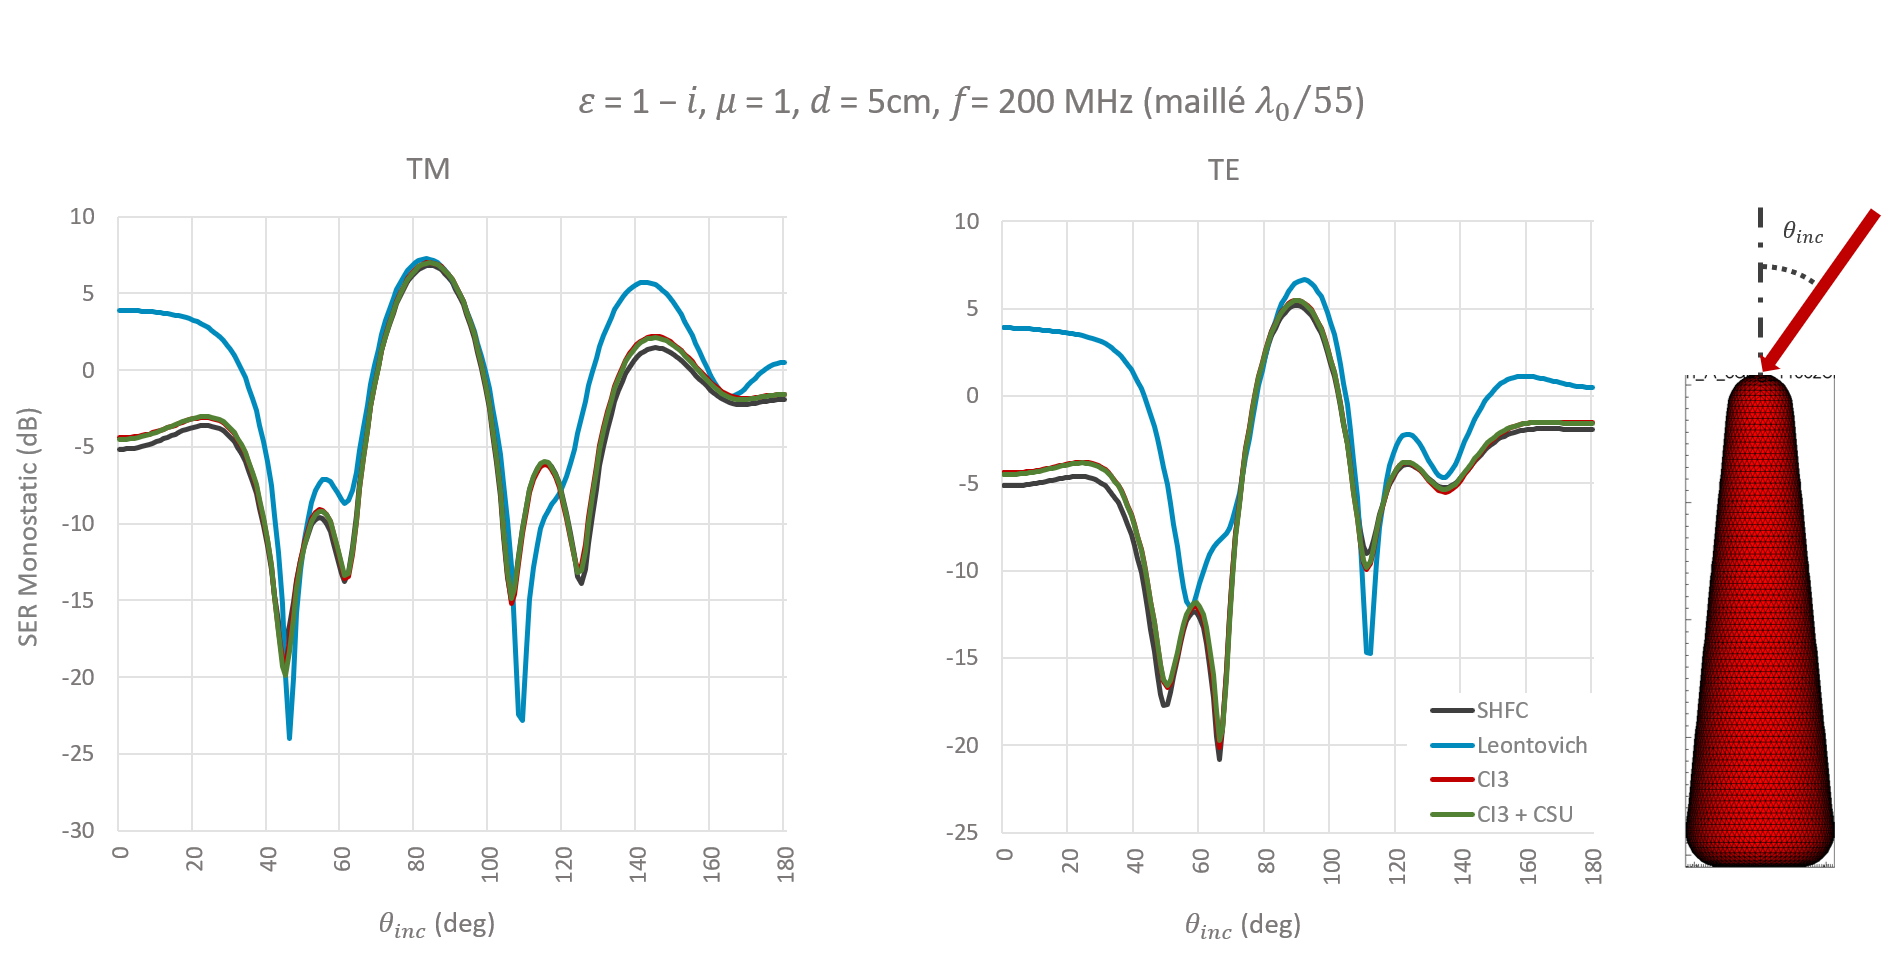
\includegraphics[width=\textwidth]{images/ser/cone_sphere_mono.png}
    \caption{SER monostatique d'un cône sphère par équations intégrales couplées avec une CIOE où les coefficients sont calculés dans le cadre de l'approximation du plan tangent.}
    \label{fig:ser:cone-sphere-mono-M1}
  \end{figure}


  \begin{figure}[!hbt]
    \centering
    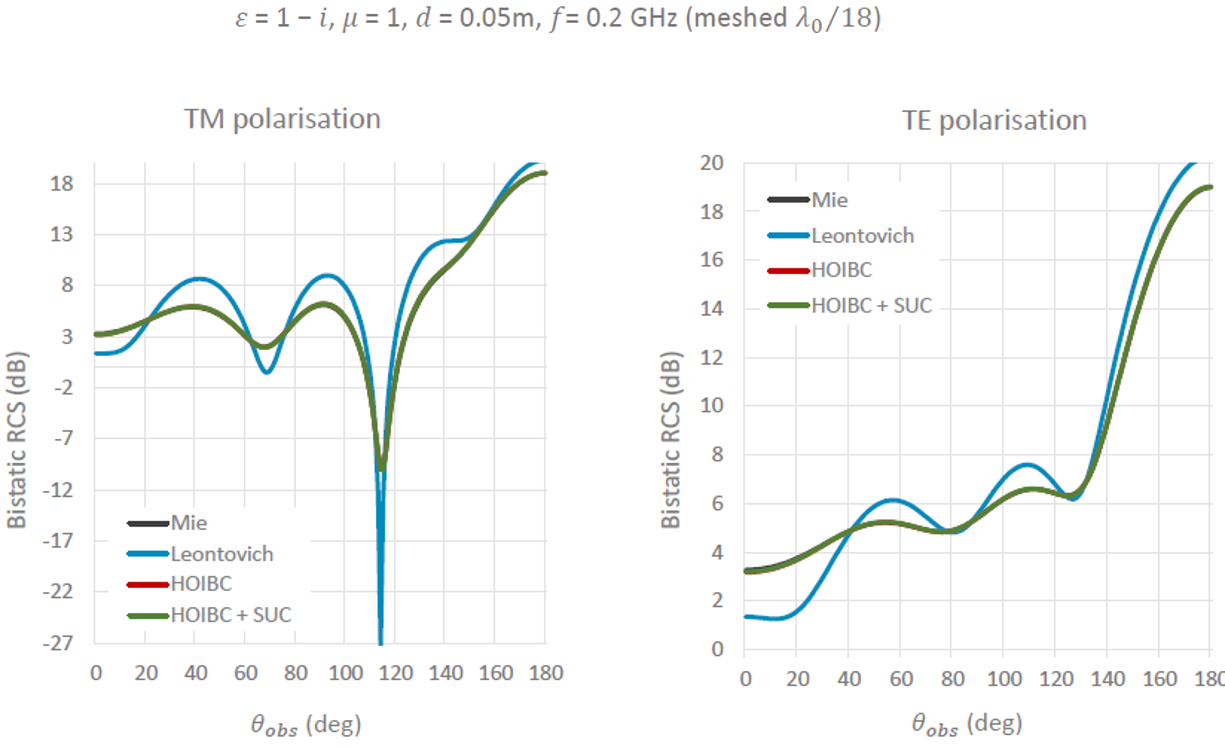
\includegraphics[width=\textwidth]{images/ser/sphere_bis.png}
    \caption{SER bistatique d'une sphère par équations intégrales couplées avec une CIOE où les coefficients sont calculés dans le cadre de l'approximation du plan tangent.}
    \label{fig:ser:sphere-bis-M1}
  \end{figure}

  Ces figures montrent que la SER calculée par EI avec CIOE est très proche de la solution de référence, calculée par un code axis symétrique de type équations intégrales avec éléments finis avec maillage des matériaux.

